\chapter{Model-Experiment Comparison}\label{c:compare}

In this chapter we'll discuss some general methods for comparing model predictions with experimental observations.  We are interested in being able to answer the questions, \emph{How good is the model?}, or more specifically, \emph{How good is the model at predicted the behavior of the physical system?}  We'll also present examples that show how these general concepts can be applied to particular models and experiments such as static and first-order models of physical systems like bending beams and temperature sensors.

We can make both \glspl{qualitative comparison} and \glspl{quantitative comparison} between model predictions and experimental data.  A qualitative comparison is based on subjective criteria such as does the time-response of our model ``look like'' the observed experimental data.  Qualitative evaluation is important, but it can only get us so far. As engineers we'll want to quantify our evaluation to put the comparison in subjective, numerical terms (hopefully with units!).  


\section{Quantitative Comparison}

\renewcommand{\ThisFigWidth}{0.3}
\begin{figure}[th!]
\centering
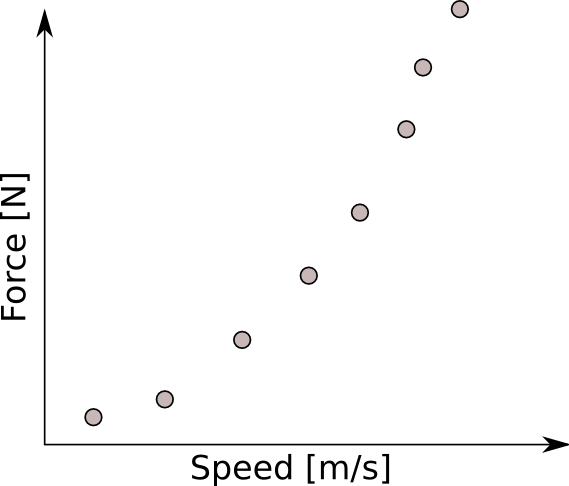
\includegraphics[width=\ThisFigWidth\textwidth]{model_fit_data.png}
\caption{Graph of our empirical measurements of pulling something through some fluid and measuring the drag force.  The individual data points are shown as circles.}
\label{f:modeldata}
\end{figure}

Let's consider an example.  Imagine we are measuring the drag force on something (a boat, surfboard, fish, diver, hang glider, etc.) as it moves through a fluid (air, water, mercury, etc.).  We pull our thing through our fluid at a few different speeds and measure the force.  If we plot our data it might look something like Figure~\ref{f:modeldata}.  Now that we have data, we might consider what type of (mathematical) model would be a good representation (or fit) to the model.  One thing we might try is to consider a \emph{linear model}, i.e., we are proposing that there is linear relationship between speed and drag force.  To be more specific, we are proposing that the function $F_{\mathrm{drag}}=m(V)$ could be a ``good'' representation of our observation.
\begin{figure}[hb!]
\centering
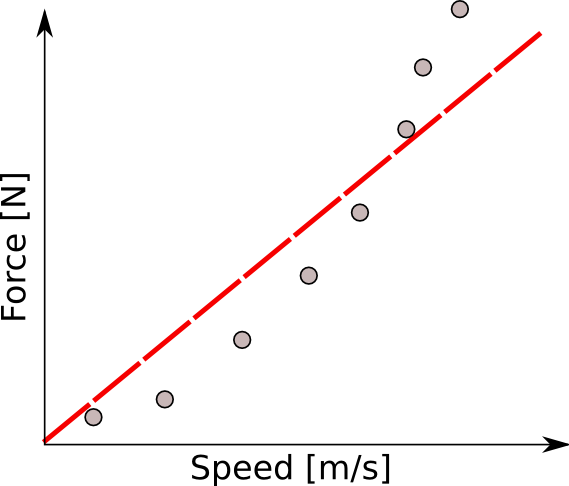
\includegraphics[width=\ThisFigWidth\textwidth]{model_fit_line.png}
\caption{Graph of our empirical measurements with a notional linear model.  The data (circles) and the linear model (red dashed line) are shown together.}
\label{f:modelline}
\end{figure}
Based on our data and our proposed model we could then come up with a value for the $m$ term in our model.  Figure~\ref{f:modelline} illustrates what this might look like.  Qualitatively this model ``looks pretty good'', but...

Alternatively, we might consider a different model.  Perhaps we could try a \emph{quadratic model} of the form $F_{\mathrm{drag}}=c(V^2)$.  Again, there is just one parameter in our model ($c$) that we'll need to choose so that the model and the data are similar. If we can find a reasonable quadratic coefficient we might get something that looks like Figure~\ref{f:modelquad}.  Based on this graph we could conclude, qualitatively, that the quadratic model is a ``better fit'' than the linear model.  We could also conclude that the error between the quadratic model and the data is ``small'', but we can't really get beyond these qualitative explanations.

\begin{figure}[bh!]
\centering
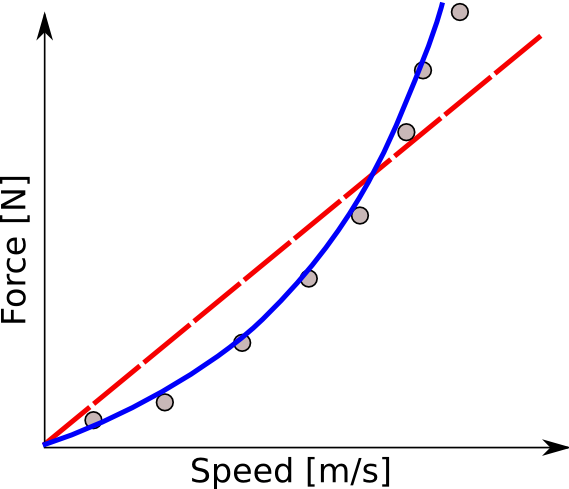
\includegraphics[width=\ThisFigWidth\textwidth]{model_fit_quad.png}
\caption{Graph of our empirical measurements with a notional linear and quadratic models.  The data (circles), linear model (red dashed line) and quadratic model (solid blue line) are shown together.}
\label{f:modelquad}
\end{figure}


\section{Quantitative Comparison}
Quantitative comparisons are based on \glspl{metric} (also known as a \emph{figure of merit}).  The metric is the numerical quantity (or quantities) that we are using to evaluate our comparison.  The type of model and experiment involved in the comparison of often dictates the types of metrics available.  In this section we'll present a few metrics that are useful for comparing the mathematical models and experiments typical in dynamic, mechanical systems.

\subsection{Simple Statistics}
We'll start with some simple (and hopefully familiar) statistical metrics.  Let's reconsider our example form Chapter~\ref{c:measure}, but this time we'll pretend we have a model.  Our ``model'' in this case is just a single prediction for the length of the fish we caught: $\hat{L}=\unit[1.0]{m}$.  (I'm not sure how we made this prediction, but we did.)  

Once we reel in our actual fish (our experiment) we use our digital ruler to make a series of measurements that we can summarize in Table~\ref{t:fishdata}. 
\begin{table}[bt!] 
\renewcommand{\arraystretch}{1.2}
\caption{Fishy Data}
\label{t:fishdata}
\centering
\begin{tabular}{|c|c|}\hline
Run & $L_i$ [m] \\ \hline \hline
1 & 0.76 \\ \hline
2 & 1.18 \\ \hline
3 & 1.17 \\ \hline
4 & 0.96 \\ \hline
5 & 1.48 \\ \hline
\end{tabular}
\end{table}
Remember, we are trying to compare our model ($\hat{L}$) with our data ($L_i$).  What could we say qualitatively?  We might say that is ``looks pretty good'', but that is very subjective.  One of our measurements is almost 50\% higher than our model prediction.  Is that ``pretty good'', ``fair'', ``poor'' or ``terrible''?

Luckily, we don't really have to make that decision.  Instead we can quantify the comparison.  One easy statistical quantity we can use is the \gls{sample mean}
\begin{equation}\label{e:mean}
\bar{L} = \frac{1}{N}\sum_{i=1}^{N} L_i
\end{equation}
where $N$ is the number of samples (5) and $\bar{L}$ is the sample mean.  We might use the MATLAB \texttt{mean()} command to calculate $\bar{L}=\unit[1.11]{m}$.  Now we have a simple quantitative comparison, and we can say something like, ``The predicted value of $L$ was \unit[1.0]{m} and the sample mean of the measured length was \unit[1.11]{m} based on 5 samples, indicating an 11\% difference between the model and the experiment.''  As an engineer, this is a much more satisfying result that the comment that the ``data looks pretty close''---true?

Another simple statistic we can use to quantify our results is the \gls{sample standard deviation},
\begin{equation}\label{e:std}
\sigma_{L}=\sqrt{\frac{1}{N-1}\sum_{i=1}^{N}\left(L_i-\bar{L}\right)^2}.
\end{equation}
The standard deviation specifies how much variability in our data, indicating how much we can trust individual measurements.  We might use the MATLAB \texttt{std()} function to calculate the standard deviation of our measurements as $\sigma_L=\unit[0.24]{m}$, indicating that the expected variability in our measurements is roughly 24\% of the modeled value.  

\begin{table}[bt!] 
\renewcommand{\arraystretch}{1.2}
\caption{Summary of our fishy results}
\label{t:fishdata}
\centering
\begin{tabular}{|l|c|}\hline
Result & Value \\ \hline \hline
Predicted Length ($L$) & \unit[1.0]{m} \\ \hline
Mean Measured Length ($\bar{L}$) & \unit[1.11]{m} \\ \hline
Percent Difference: Model/Experiment & 11\% \\ \hline
Standard Deviation of Length Measurement ($\sigma_L$) & \unit[0.24]{m} \\ \hline
\end{tabular}
\end{table}

It is important to note a few things about our first example of quantitative comparisons:
\begin{itemize}
\item Our comparisons take the form of specific metrics
\item Our metrics have both numbers and engineering units
\item We can avoid having to make subjective judgments such as ``good'' or ``better''.
\end{itemize}

\subsection{Model Coefficients}
The previous simple statistics work well for scalar measurements where the underlying model is static (a single value).  However, in this book we are more interested in dynamic models and systems that change with time.  One way we can quantify these comparisons is by contrasting the predicted model coefficients with model coefficients based on our experiments.  

Let's consider an example based on our first-order model step response from Section~\ref{s:firststep}.  Let's assume we've come up with the mathematical model
\begin{equation}
\frac{dy(t)}{dt} + \frac{1}{\tau}y(t) = f(t),
\end{equation}
and we've predicted the time-constant is $\tau=\unit[10.0]{s}$ and the steady-state value is $Y_{ss}=\unit[100]{V}$.  Based on our model we can predict the step response as 
\begin{equation}\label{e:steppred}
y(t) = Y_{ss}\left(1-e^{-t/10.0}\right).
\end{equation}
Now we go into the lab and do a set of three experiments to magically measure the step response of our system.  If we graph our predicted response (\ref{e:steppred}) alongside our experimental observations we might get a plot similar to Figure~\ref{f:firstmodelex}.
\renewcommand{\ThisFigWidth}{0.4}
\begin{figure}[th!]
\centering
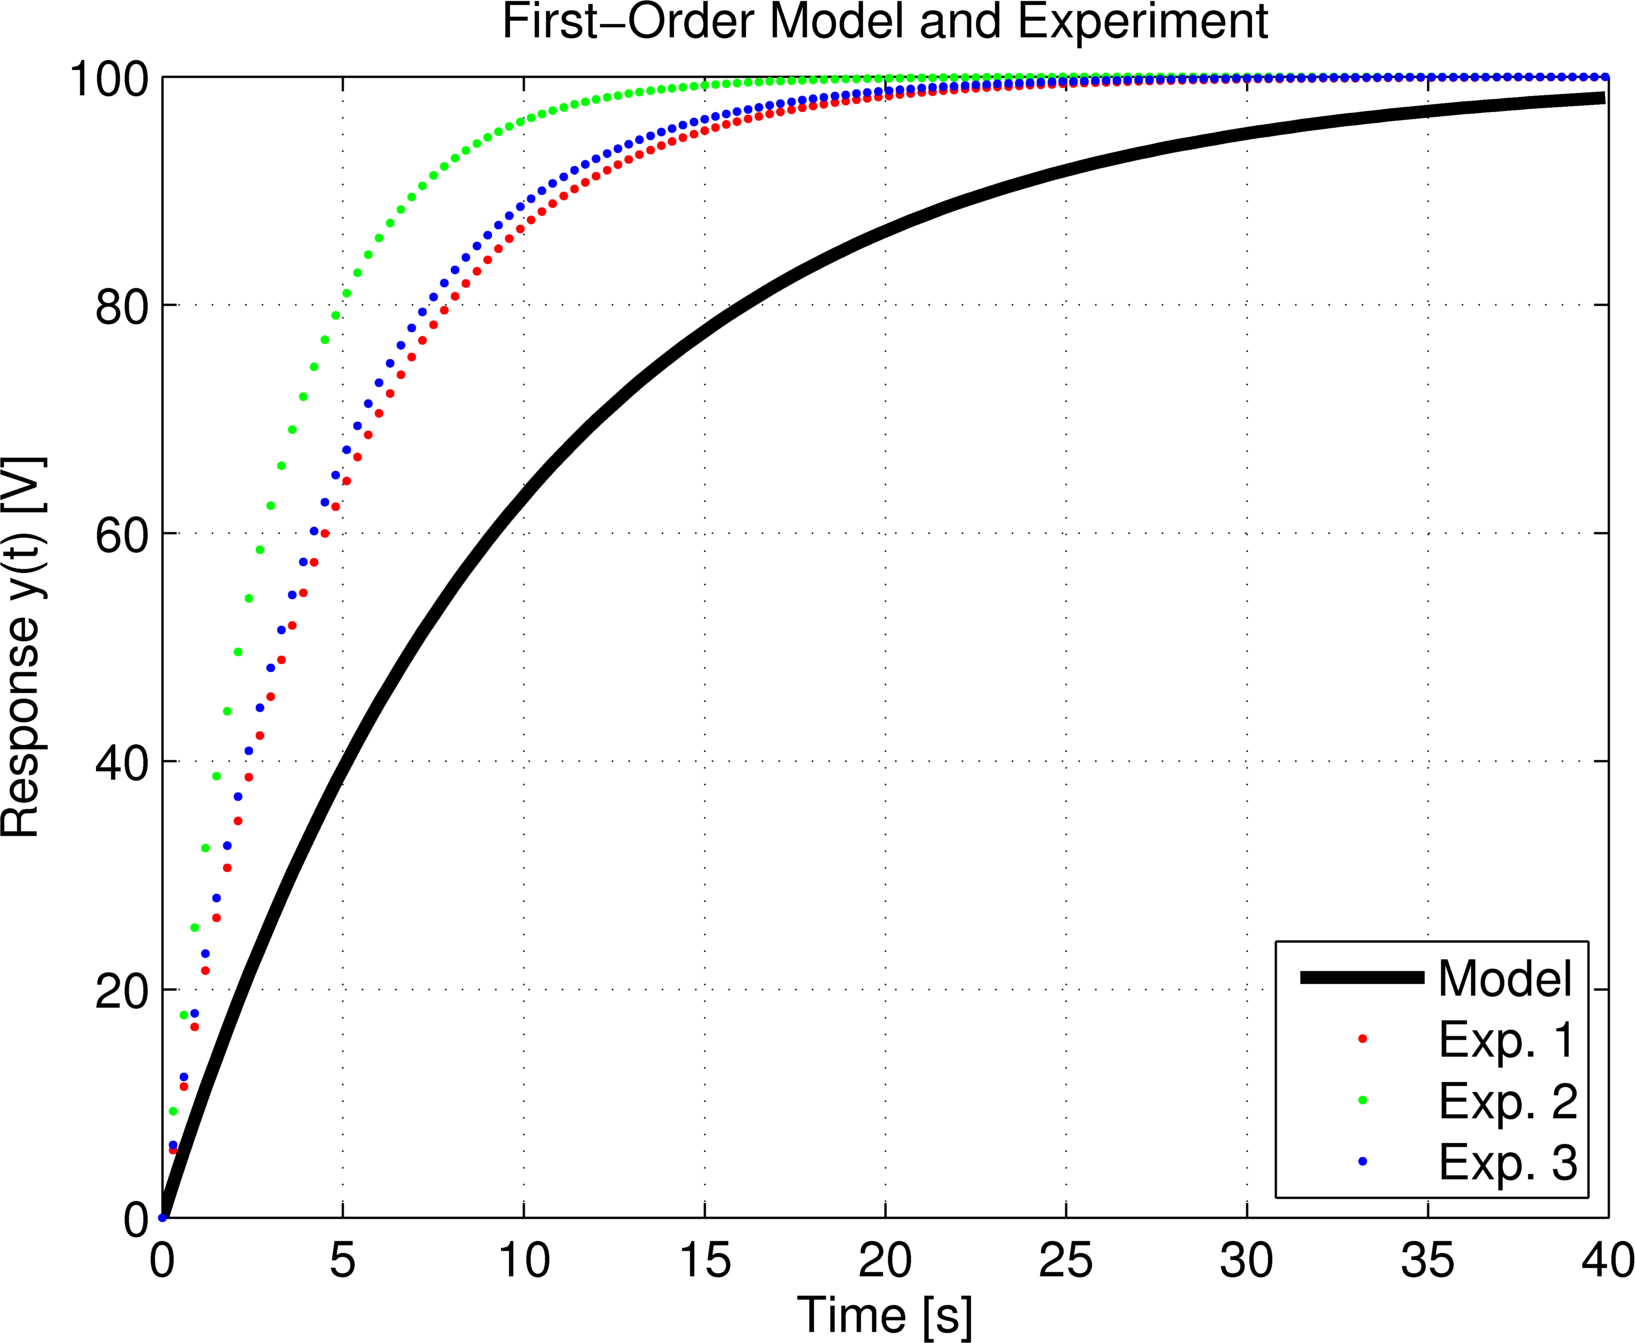
\includegraphics[width=\ThisFigWidth\textwidth]{first_modelex.png}
\caption{Illustration of our model prediction and experimental measurements.}
\label{f:firstmodelex}
\end{figure}
We can immediately make the following important qualitative comparisons:
\begin{itemize}
\item The model predicted steady-state response appears to agree with the empirical steady-state response.
\item The model predicted time constant appears to be larger than the experimentally measured time constant.
\end{itemize}
But, how do we quantify these comparisons?

One way to quantify the agreement between the model and the experimental results is to calculate a time constant based on the assumption that our physical experiment behaves like a first-order mathematical model. (Be careful here, a physical system does not have a time constant; only mathematical models have time constants!)  For each experimental trial we can estimate a time constant for the system.  Then we can compare the mean experimental time constant to the predicted time constant from the model and summarize the results in a table.
\begin{table}[bt!] 
\renewcommand{\arraystretch}{1.2}
\caption{Summary of our model predictions and experimental results}
\label{t:timec}
\centering
\begin{tabular}{|l|c|}\hline
Result & Value \\ \hline \hline
\textbf{Predicted Time Constant} & \textbf{\unit[10.0]{s}} \\ \hline
Experimental Time Constant: Run 1 & \unit[4.2]{s} \\ \hline
Experimental Time Constant: Run 2 & \unit[4.5]{s} \\ \hline
Experimental Time Constant: Run 3 & \unit[2.8]{s} \\ \hline
\textbf{Experimental Time Constant: Mean} & \textbf{\unit[3.8]{s}} \\ \hline
Difference, Model vs. Exp. Time Constant & \unit[6.2]{s} \\ \hline
\textbf{Percent Error} & \textbf{62\%} \\ \hline
\end{tabular}
\end{table}

One thing to be specific about is how we calculate the \emph{percent error} in Table~\ref{t:timec};
\[
\%\,\mathrm{Error}=\frac{|\mathrm{Experimental}-\mathrm{Theoretical}|}{\mathrm{Theoretical}}.
\]
